\documentclass[letterpaper]{article}
\usepackage[pass]{geometry}
\usepackage{hyperref}
\usepackage{tabularx}
\usepackage{array}
\usepackage{siunitx}
\usepackage{graphicx}
\graphicspath{ {./images/} }

\title{Controller Area Network (CAN) and QFSAE}
\author{Ethan Peterson}
\date{\today}

\begin{document}

\maketitle

\section{CAN Bus Protocol}

\subsection{Background}
Controller Area Network (CAN) is a communications protocol that is standard for
electronics in the automotive industry. The protocol was introduced by the
Society of Automotive engineers (SAE) in 1986. CAN is primarily used for
communication between different electronics systems in different locations on
the car. For instance, sensor systems on the back of vehicle would be able to
read data from the Engine Control Unit (ECU). In the case of the team's car, the
ECU is the primary CAN device that other systems communicate with. The ECU
provides a variety of metrics about the engine such as RPM, throttle position,
ignition angle and many more. These metrics are read from the ECU over CAN by
using their CAN ID. Each message must have a unique ID from the IDs in use by
other devices on the car. It is also important to note that only one message can
be on a CAN bus at a time. Messages with more ``dominant" IDs will take
precedence on the bus. As a result, there must be careful consideration when
selecting an ID for a certain message depending on its priority overall.

\subsection{Data Transmission and Addressing}
CAN is two wire half-duplex serial based communication protocol. Half duplex
means that the CAN bus can only be used to send or receive messages in an
alternating fashion and not at the same time as with full-duplex protocols. CAN
messages consist of an identifier (CAN ID) and a data frame. There are several
standards for the size of the message frames. The ECU on the QFSAE car
implements the Society of Automotive Engineers (SAE) J1939 standard. This
standard uses 29 bit message identifiers and 64 bit data frames. Since CAN is
half-duplex, only one message can be on the bus at a time. However, CAN can
still be used to create large networks of CAN devices despite this through
its implementation of a priority bus. CAN defines ``dominant" and ``recessive"
bits where logical 0 is dominant. This allows to CAN to resolve conflicts on the
bus. The table below summarizes this process.

\begin{center}
  \begin{table}
  \begin{tabular}{c|c|c|c|c|c|}
    \cline{2-6}
      & \multicolumn{4}{c}{CAN ID Bits} & \\
    \cline{2-6}
      & Start Bit & 3 & 2 & 1 & 0\\
    \cline{1-6}
      \multicolumn{1}{|c|}{Node 3} & 0 & 0 & 0 & 0 & 1 \\
    \cline{1-6}
      \multicolumn{1}{|c|}{Node 4} & 0 & 0 & 1 & Stopped Transmitting & N/A \\
    \cline{1-6}
      \multicolumn{1}{|c|}{CAN Bus Data} & 0 & 0 & 0 & 0 & 1 \\
    \hline
  \end{tabular}
  \caption{
  \label{tab:Address Conflict Resolution}
    Demonstrating how CAN chooses the most ``dominant" ID on the bus in the
    case of a conflict between messages.
  }
  \end{table}
\end{center}

As a result of 0 being the dominant bit on the bus it is the smallest
CAN IDs that have the highest priority on the bus. This property of the bus must
be considered when selecting CAN IDs for custom messages outside of those
broadcast by the ECU. For example, a message indicating to the dash that a gear
shift happened is likely of a higher priority than updating the RPM.

\subsection{Wiring}
CAN consists of a two wire interface where the first two nodes connected to one
another should have two 120\si{\ohm} terminating resistors connected on either
end of the bus. Nodes are defined as devices connected to the bus which can send
or receive CAN messages. The diagram below is an example CAN network with three nodes.

\begin{center}
  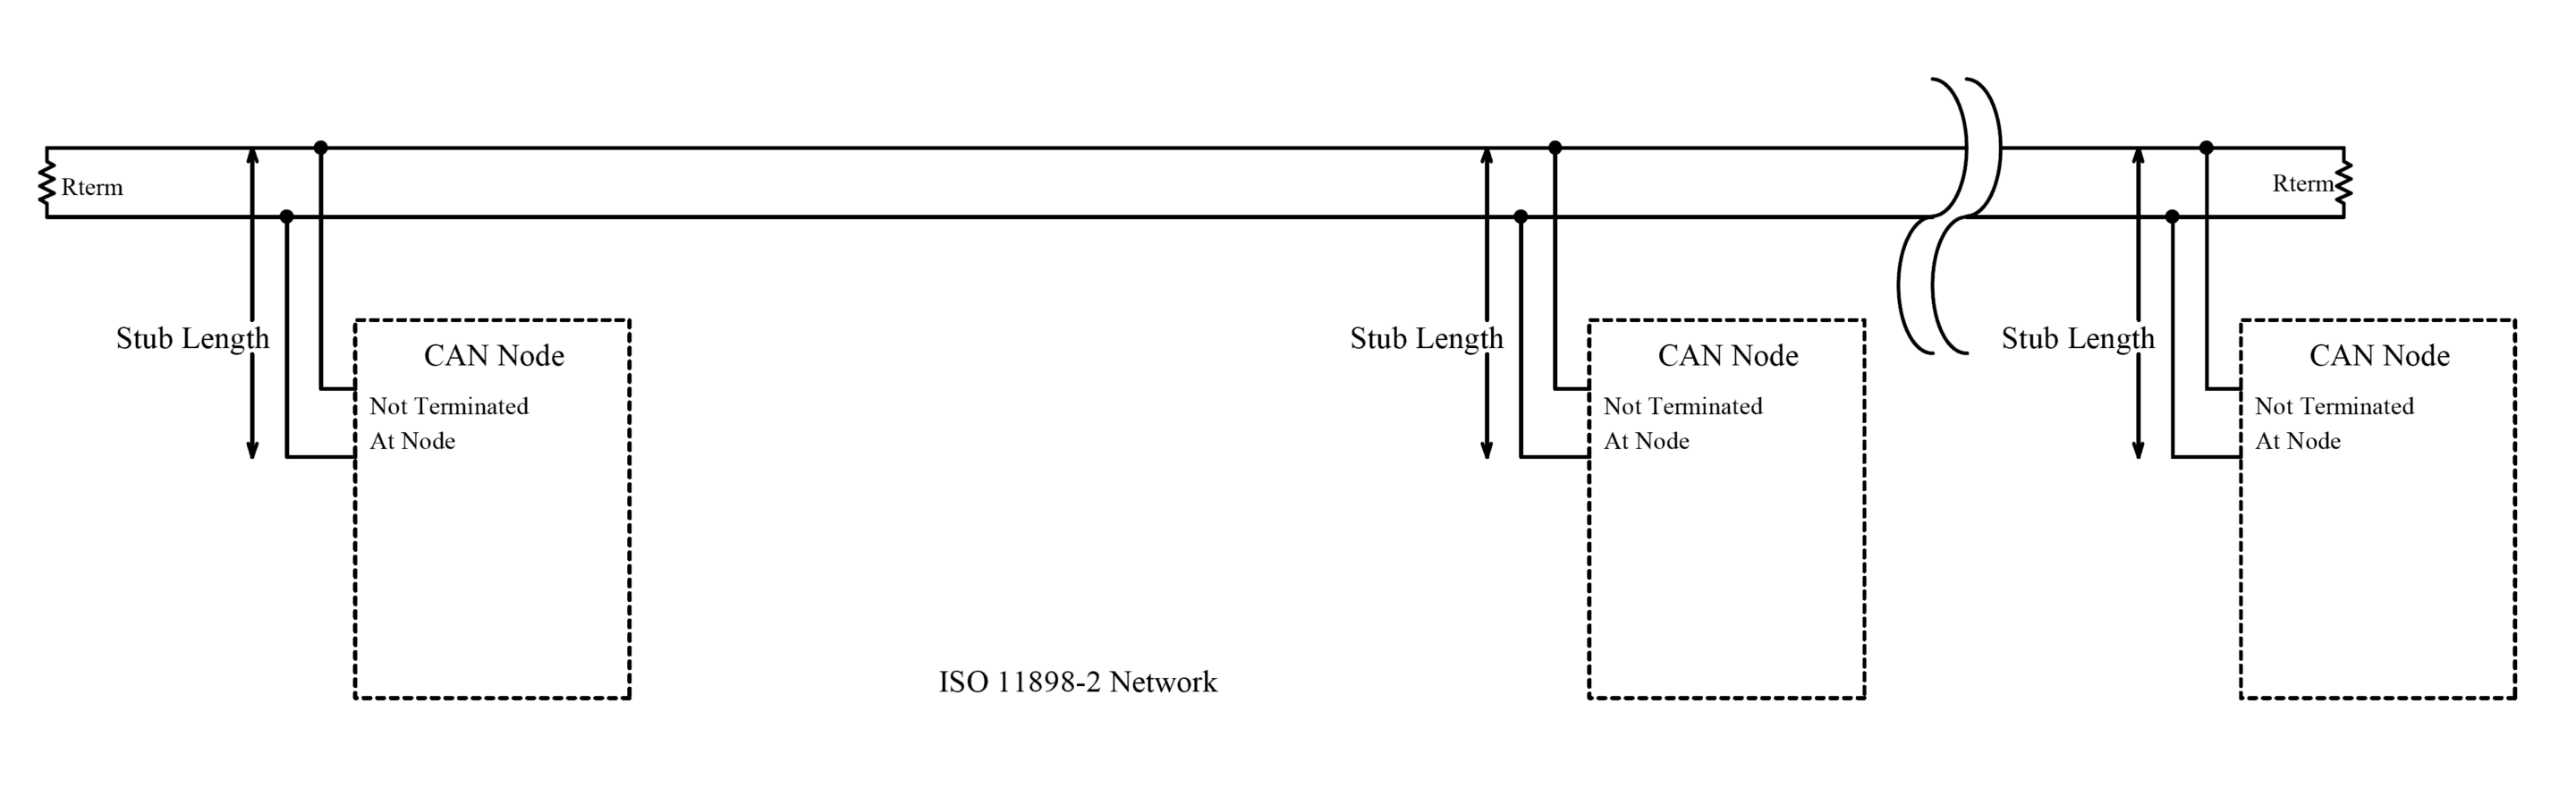
\includegraphics[width=\textwidth]{CAN-network-diagram}
\end{center}

In the case of the Formula car, The ECU has a terminating resistor and so does
the end of the car's CAN line where the CAN to USB dongle is found. Thus,
additional CAN peripheral should omit the terminating resistor to keep the bus
functioning properly.

\end{document}
